\documentclass[10pt,a4paper]{article}

\usepackage{siunitx} % Provides the \SI{}{} and \si{} command for typesetting SI units
\usepackage{graphicx} % Required for the inclusion of images
\usepackage{caption}
\usepackage{subcaption}
\usepackage{natbib} % Required to change bibliography style to APA
\usepackage{amsmath} % Required for some math elements 
\usepackage{listings}
\usepackage{fancyvrb}
\usepackage[a4paper]{geometry}
\usepackage{float}
\usepackage{hyperref}
\usepackage{natbib}
\bibliographystyle{plain}


%------------------------------------------------------------------
% a couple horizontal bars to delimit embedded code
% the width suits the page size set above and
% the mathmode eliminates spaces between the three elements
\newcommand{\topbar}{\ensuremath{
    \rule{0.1mm}{2.0mm} \rule[2.0mm]{159.5mm}{0.1mm} \rule{0.1mm}{2.0mm}
}}
\newcommand{\bottombar}{\ensuremath{
    \rule{0.1mm}{2.0mm} \rule{159.5mm}{0.1mm} \rule{0.1mm}{2.0mm}
}}
\newcommand{\topbarshort}{\ensuremath{
    \rule{0.1mm}{2.0mm} \rule[2.0mm]{149.5mm}{0.1mm} \rule{0.1mm}{2.0mm}
}}
\newcommand{\bottombarshort}{\ensuremath{
    \rule{0.1mm}{2.0mm} \rule{149.5mm}{0.1mm} \rule{0.1mm}{2.0mm}
}}
%------------------------------------------------------------------


% \setlength\parindent{0pt} % Removes all indentation from paragraphs

% set Header of Report
\title{PotentialFlow.py a Potential Flow Solver and Visualizer}
%\subtitle{}
\author{Mechanical Engineering Technical Report 2015/08 \\ 
Ingo \textsc{Jahn} \\ 
School of Mechanical and Mining Engineering \\ 
The University of Queensland.}
\date{\today} 

\begin{document}

\maketitle 

\begin{abstract}
\verb'Potential_Flow.py' is a simple teaching and analysis tool for 2-D Potential Flow. 
It is a collection of code, that allows the construction of simple flow fields that meet the Potential Flow governing Equations.
A range of plotting and visulisation tools are included. 
\\ \\
This report is a brief userguide and example book. 
\end{abstract}

% \tabelofcontents

%%%%%%%%%%%%%%%%%%%%%%%%%%%%%%%%%%%%%%%%%%%%%%%%%%%%%%
%%%%%%%%%%%%%%%%%%%%%%%%%%%%%%%%%%%%%%%%%%%%%%%%%%%%%%
\section{Introduction}
Potential Flow is a simple but powerful analysis approach to simulate inviscid flow. 
This report is the userguide for \verb'Potential_Flow.py' a tool to analyse simple 2-D flows together with a selection of plotting and post-processing tools.
The code allows the flow-fields consisting of the following building blocks to be analysed: 
Uniform Flow, Sink/Source, Irrotational Vortex, Doublet. \\
The post-processing tool allows the generation of streamline plots, velocity contour plots, and pressure contours.
In addition post-processing tools are included to extract point data and data along user-defined lines. 


%%%%%%%%%%%%%%%%%%%%%%%%%%%%%%%%%%%%%%%%%%%%%%%%%%%%%%
\subsection{Compatibility}
\verb'Potential_Flow.py' is written in python. 
The following packages are required:
\begin{itemize}
\item \verb'python 2.7' - any standard distribution
\item\verb'numpy'
\item\verb'matplotlib' 
\end{itemize}

%%%%%%%%%%%%%%%%%%%%%%%%%%%%%%%%%%%%%%%%%%%%%%%%%%%%%%
\subsection{Citing this tool}
When using the tool in simulations that lead to published works, it is requested that the following works are cited:
\begin{itemize}
\item Jahn, I. (2015), PotentialFlow.py a Potential Flow Solver and Visualizer, {\it Mechanical Engineering Technical Report 2015/08},  The University of Queensland, Australia \\
\end{itemize}

%%%%%%%%%%%%%%%%%%%%%%%%%%%%%%%%%%%%%%%%%%%%%%%%%%%%%%
%%%%%%%%%%%%%%%%%%%%%%%%%%%%%%%%%%%%%%%%%%%%%%%%%%%%%%
\section{Distribution and Installation}
\verb'Potential_Flow.py' is distributed as part of the code collection maintained by the \emph{CFCFD Group} at the University of Queensland \citep{cfcfdpage:2015}. 
This collection is free software: you can redistribute it and/or modify it under the terms of the GNU General Public License as published by the Free Software Foundation, either version 3 of the License, or any later version. 
This program collection is distributed in the hope that it will be useful, but WITHOUT ANY WARRANTY; without even the implied warranty of MERCHANTABILITY or FITNESS FOR A PARTICULAR PURPOSE. 
See the GNU General Public License for more details \url{http://www.gnu.org/licenses/}.
\\
Alternatively the code is included in the Appendix.

%%%%%%%%%%%%%%%%%%%%%%%%%%%%%%%%%%%%%%%%%%%%%%%%%%%%%%
\subsection{Modifying the code}
The working version of \verb'Potential_Flow.py' is installed in the \verb'$HOME/e3bin' directory.
If you perform modifications or improvements to the code please submit an updated version together with a short description of the changes to the authors.
Once reviewed the changes will be included in future versions of the code. 


%%%%%%%%%%%%%%%%%%%%%%%%%%%%%%%%%%%%%%%%%%%%%%%%%%%%%%
%%%%%%%%%%%%%%%%%%%%%%%%%%%%%%%%%%%%%%%%%%%%%%%%%%%%%%
\clearpage
\section{Using the Tool: 5-minute version for experienced python Users}

%%%%%%%%%%%%%%%%%%%%%%%%%%%%%%%%%%%%%%%%%%%%%%%%%%%%%%
\subsection{5-minute version for experienced python Users}
If you understand python, including classes and know how the potential flow building blocks work, this is for you. 

\begin{enumerate}
\item Find the \verb'if __name__ == "__main__":' section of file and then adjust the following parts.
\item Create a list of instances of the various building block classes (e.g. \verb'A1 = Uniform(1.0,)' ). 
A full list of options is available in section~\ref{S_building_blocks}.
\item Create an instance of the FlowField class. \verb'T = PlotPotentialFlow()'
\item (Optional) Adjust the size of the flow-field. \verb'T.size(x0=0.0, x1=1.0, y0=0.0, y1 = 1.0)'
\item Solve the flow-field. \verb' T.calc([List],n=100)', where \verb'[List]' is a list of building block instances from step 2.
\item Plot the results using private functions of the FlowField class (e.g. \verb'T.plotStreamlines()') \\
(make sure \verb'plt.show()' is included to display graphs)
\item Evaluate point data or extract line data
\item Run using the command: \verb'python Potential_Flow.py' \\
Filename may need to be adjusted to incorporate version)   
\end{enumerate}



%%%%%%%%%%%%%%%%%%%%%%%%%%%%%%%%%%%%%%%%%%%%%%%%%%%%%%
%%%%%%%%%%%%%%%%%%%%%%%%%%%%%%%%%%%%%%%%%%%%%%%%%%%%%%
\section{Using the Tool: Detailed}

%%%%%%%%%%%%%%%%%%%%%%%%%%%%%%%%%%%%%%%%%%%%%%%%%%%%%%
\subsection{Creating your Flow field}
In potential flow different flow feature {\it building blocks}, that full-fill Laplace's equation by themselves, are superimposed (added) in order to generate complex flow-field solutions. 
The first part of involves setting creating such building blocks that can be combined to create a complex flow-field.
\\ \\
\noindent
{\huge Step: 1}\\
Find  \verb'if __name__ == "__main__":', the part of the file that will be executed if the file is run from the command line.
\\ \\

\noindent
{\huge Step: 2}\\
Create a list of building blocks that you want to use for your flow. 
The result should look something like the following for Uniform Flow $+$ a Source:
 
\noindent
\topbar
\begin{lstlisting}
if __name__ == "__main__":

    # List of Building Blocks 
    # Uniform Flows  
    A1 = UniformFlow(5.,0.)
    # Sources
    D1 = Source(0.5,0., 5.)
\end{lstlisting}
\bottombar

The possible options for building blocks, together with detailed descriptions are described in section~\ref{S_building_blocks}.


%%%%%%%%%%%%%%%%%%%%%%%%%%%%%%%%%%%%%%%%%%%%%%%%%%%%%%
\subsubsection{Building Blocks}\label{S_building_blocks}
Currently the following Building Blocks are supported.

\begin{description}
\item[Uniform Flow:] \verb'UniformFlow(u,v)' \\ This creates a uniform flow with the velocity components $u$ and $v$ in the x- and y-direction respectively. 
The streamlines for the flow-field are shown in Fig.~\ref{F_Uniform_Flow}. \\
The streamfunction is defined as: 
\begin{equation}
\Psi = u \, y - v \, x
\end{equation}

\item[Source:] \verb'Source(x0,y0,m)' \\ This generates a source (use -ve $m$ for sink) located at the position defined by $(x0,y0)$. 
Streamlines for the flow-field are shown Fig.~\ref{F_source}. \\
The streamfunction is defined as: 
\begin{eqnarray}
\noindent \theta &=& \tan^-1 \left( \frac{ y -y0}{x-x0} \right)\\
\Psi &=& \theta \frac{m}{2 \, \pi}
\end{eqnarray}

\item[Vortex:] \verb'Vortex(x0,y0,K)' \\ This generates an irrotational vortex of strength $K$, with the core locates at $(x0,y0)$. 
Streamlines for the flow-field are shown Fig.~\ref{F_vortex}. \\
The streamfunction is defined as: 
\begin{eqnarray}
\noindent r &=&  \left[ \left( x-x0 \right)^2  +  \left( y-y0 \right)^2  \right]^{\frac{1}{2}} \\
\Psi &=& -K \, \ln r
\end{eqnarray}

\item[Doublet:] \verb'Doublet(x0,y0,a,U_inf)' \\ 
This generates the flow field known as a doublet. 
This is generated if a source and sink are brought very close together with a separation $s = \frac{a^2 \, \pi U_{\infty}}{m}$, where the $\pm m$ is the strength of the source / sink. 
The center of the doublet is located at $(x0,y0)$. 
Streamlines for the flow-field are shown Fig.~\ref{F_doublet}. \\
The streamfunction is defined as: 
\begin{eqnarray}
\Psi &=& U_{\infty} \, \left(y - y0\right) \, \frac{ - a^2}{  \left(x-x0\right)^2 + \left(y-y0\right)^2 }   
\end{eqnarray}
This doublet works only for flow in the $+x$ directions. 
For other flows modify the code or manually generate a doublet by bringing together a sourcesink aligned with the flow direction. 

\item[User\textunderscore defined:] \verb'User_Defined(x0,y0,A)' \\ 
This generates the streamlines for flow around a \SI{90}{\degree} corner, located at position. 
Streamlines for the flow-field are shown Fig.~\ref{F_User}. \\
The streamfunction is defined as: 
\begin{eqnarray}
\Psi &=& A  \,  \left(x - x0\right) \,  \left(y - y0\right)
\end{eqnarray}

\item[Name] \verb'Name(x0,y0,Var1,Var2,Var3)' \\
This is a template for future building blocks that need to be implemented. 
The block class need to have the following three functions:
	\begin{itemize}
	\item \verb'__init__(self,....)' Which is used to initialize the function
	\item \verb'evaPl(self,x,y)' Which returns the value of $\Psi$ at the point defined by the coordinates  $(x0,y0)$
	\item \verb'eval(self,x,y)' Which returns the value of the $u$ and $v$ velocity at the point defined by the coordinates  $(x0,y0)$. 
		This should be the analytical solution to $\frac{d \Psi}{dy}$ and $-\frac{d \Psi}{dx}$.
	\end{itemize}
\end{description}


\begin{figure}
\centering
\begin{subfigure}{0.32\textwidth}
    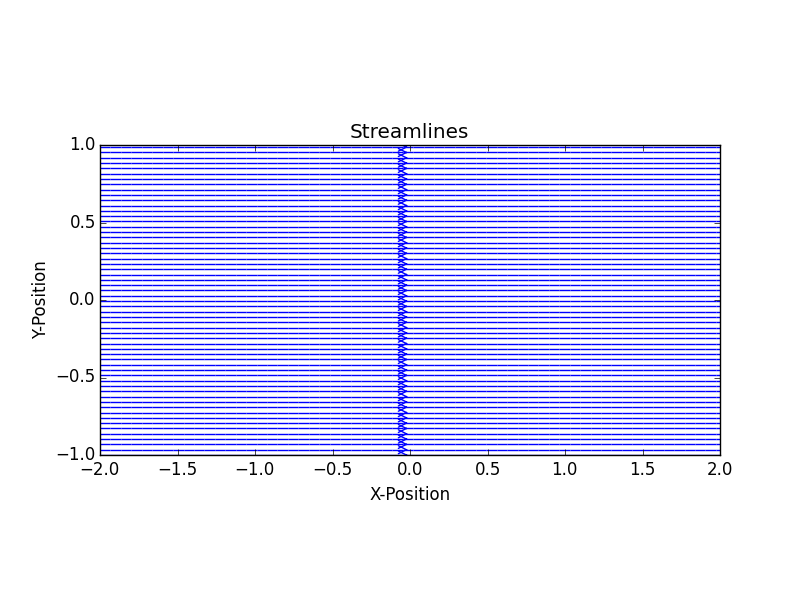
\includegraphics[width=1.0\textwidth]{Figures/Uniform}
  \caption{Uniform Flow}\label{F_Uniform_Flow}
\end{subfigure}
\hfill
\begin{subfigure}{0.32\textwidth}
    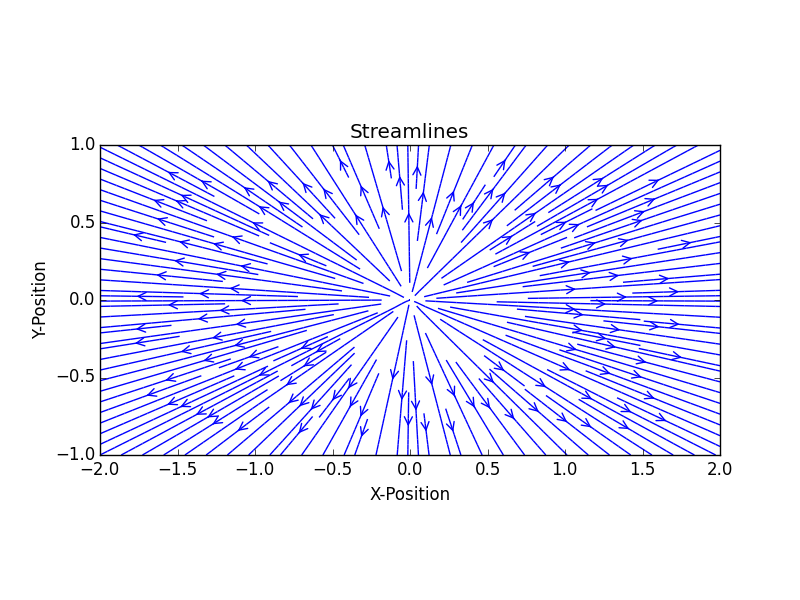
\includegraphics[width=1.0\textwidth]{Figures/Source}
  \caption{Source}\label{F_source}
\end{subfigure}
\hfill
\begin{subfigure}{0.32\textwidth}
    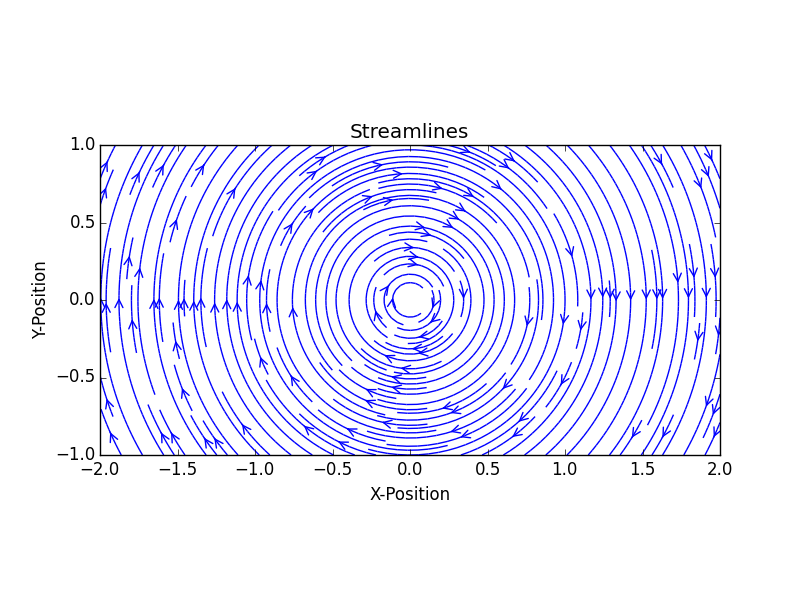
\includegraphics[width=1.0\textwidth]{Figures/Vortex}
  \caption{Vortex}\label{F_vortex}
\end{subfigure}
\\
\centering
\begin{subfigure}{0.32\textwidth}
    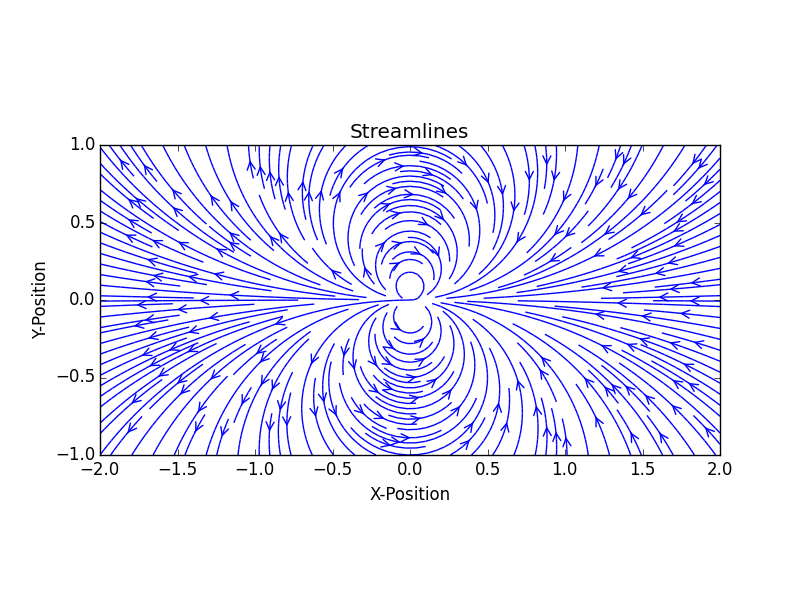
\includegraphics[width=1.0\textwidth]{Figures/Doublet}
  \caption{Doublet}\label{F_doublet}
\end{subfigure}
\begin{subfigure}{0.32\textwidth}
    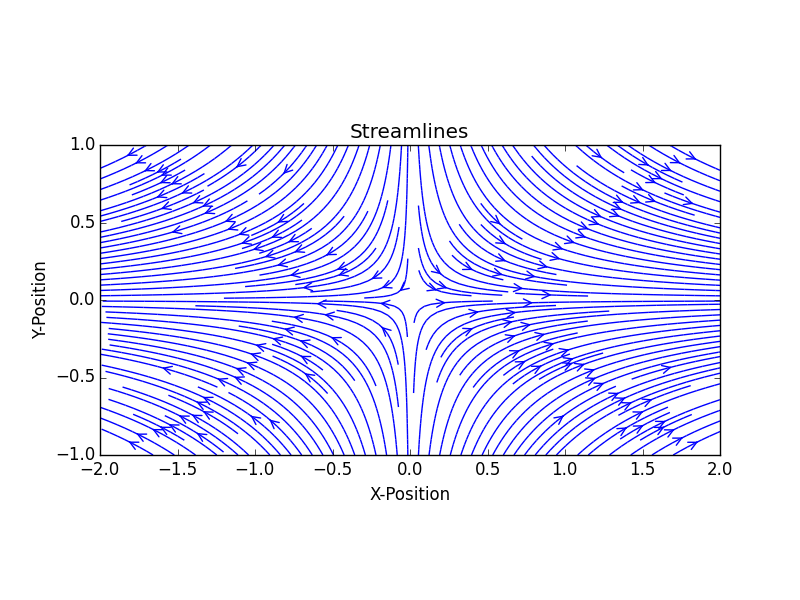
\includegraphics[width=1.0\textwidth]{Figures/User_Defined}
  \caption{User Defined}\label{F_User}
\end{subfigure}
\hfill
\caption{Building Blocks available to generate Potential Flow solutions.}
\label{F_Blocks}
\end{figure}


%%%%%%%%%%%%%%%%%%%%%%%%%%%%%%%%%%%%%%%%%%%%%%%%%%%%%%
\subsection{Creating the Flow-Field and calculating PSI, u and v}

After the building blocks have been defined, the next step is to create a flow-field area over which the Potential Flow functions will be evaluated. 
And to perform calculations to obtain $\Psi$, $u$, and $v$ over this field.
\\ \\
\noindent
{\huge Step: 3}\\
Create an instance of the PotentialFlow-field class, set the size. 
The results for an area ranging from $x = \num{-2.0}$ to $x=\num{2.0}$ and $y = \num{-1.0}$ to $x=\num{1.0}$ should look something like:

\noindent
\topbar
\begin{lstlisting}
    # Initialise instance of Plotting Function
    T = PlotPotentialFlow()   	# create instance of the PotentialFlow-field class
    # Set dimensions of Plotting area
    T.size(-2.0, 2.0, -1.0 ,1.0)   #(x_min, x_max, y_min, y_max)
\end{lstlisting}
\bottombar
\\ \\
\noindent
{\huge Step: 4}\\
Assemble a list of building blocks and evaluate these over an $N \times N$ grid spanning the area set in step 3. 
The list of blocks is generated as \verb'[ BLK-1, BLK-2, BLK-3 ]', where \verb'BLK-N' are the variable names of the different blocks. 
For flow-field consisting of Uniform Flow $+$ a Source (as per step 2) that is evaluated over a $100 \times 100$ grid the code is: (extent of the grid is set in step 3)
%(Based on area from step 4, this yields the following spacings: $\Delta x = 0.04$; $\Delta y = 0.02$)

\noindent
\topbar
\begin{lstlisting}
    # Evaluate PotentialFlow-field over a grid
    T.calc([A1,D1],n=100)   # ([List of elements], level of discretisation)
\end{lstlisting}
\bottombar


%%%%%%%%%%%%%%%%%%%%%%%%%%%%%%%%%%%%%%%%%%%%%%%%%%%%%%
\subsection{Plotting data}

Once the flow-field has been calculated, it is possible to plot fluid properties over the flow-field area defined in step 3. 
\\ \\
\noindent
{\huge Step: 5}\\
Plotting commands are exercised on the Flow-field class (e.g. \verb'T') in the above example. 
To plot streamlines and a second graph of streamlines overlayed with velocity magnitude contours, use the following code. The results are shown in Fig.~\ref{F_results_test}

\noindent
\topbar
\begin{lstlisting}
    # plot Data over flow-field area
    T.plot_Streamlines()    # create Streamline plot.
    T.plot_Streamlines_magU(100) # create plot of Streamlines + velocity magnitude

    # Make sure plots are displayed on the screen
    plt.show()
\end{lstlisting}
\bottombar

\noindent
The entire program is executed using the command \verb'python Potential_Flow.py'. 


\begin{figure}
\centering
\begin{subfigure}{0.48\textwidth}
    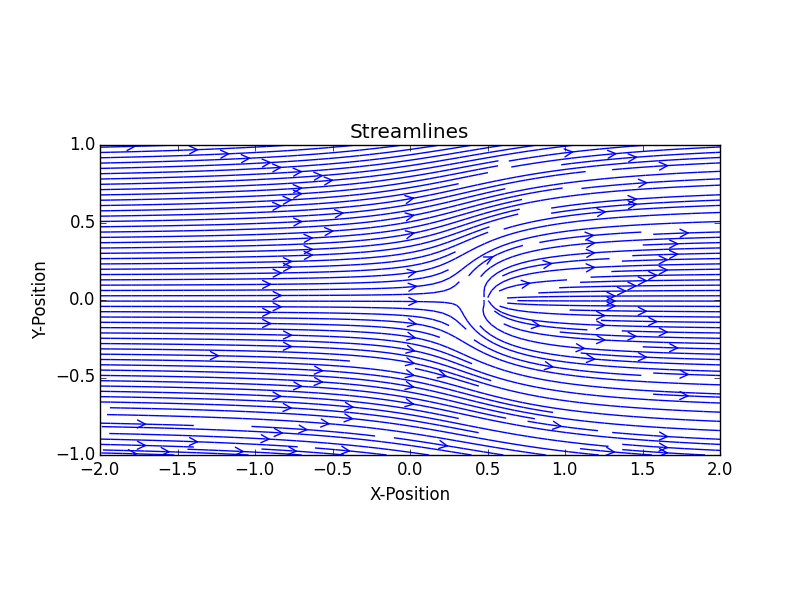
\includegraphics[width=1.0\textwidth]{Figures/Uniform_Source_SL}
  \caption{Streamlines}
\end{subfigure}
\hfill
\begin{subfigure}{0.48\textwidth}
    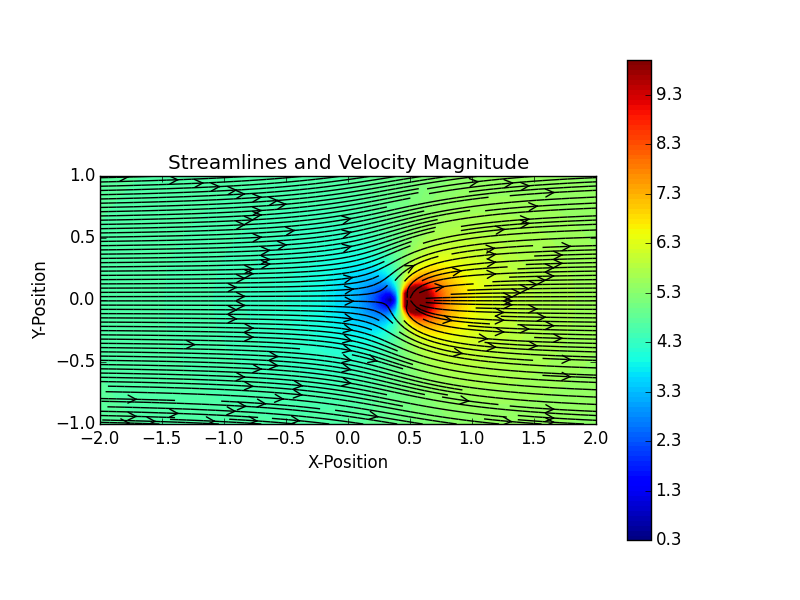
\includegraphics[width=1.0\textwidth]{Figures/Uniform_Source_SL_magU}
  \caption{Streamlines superimposed with contours of Velocity magnitude (magnitude capped at \SI{10}{\meter\per\second}).}
\end{subfigure}
\caption{Streamline and Streamline $+$ Velocity magnitude plots generated for flow-field generated by {\it UniformFlow} and {\it Source} }
\label{F_results_test}
\end{figure}

The possible options for plotting field data are described in section~\ref{S_plotting}.

%%%%%%%%%%%%%%%%%%%%%%%%%%%%%%%%%%%%%%%%%%%%%%%%%%%%%%
\subsubsection{Plotting Functions}\label{S_plotting}
The following functions extract data from the total flow-field.
They must be executed on the PotentialFlow-filed class (e.g. \verb'T') in the example above.  
In the description below \verb'NAME' is used as a generic placeholder. 
These functions must be executed after \verb'NAME.calc([List])'



\begin{description}
\item[Streamlines] \verb'NAME.plot_Streamlines()'\\
Creates a streamline plot. 
These are based on the $(u,v)$ velocity field, so while these correspond to lines of constant $\Psi$, the difference in stream function $\Psi$ between two lines is not constant. 
To obtain values of $\Psi$ use the extract point data functions (see section~\ref{S_extract})

\item[Velocity Magnitude] \verb'NAME.plot_magU(magU_max = 100., levels=20)'\\
Creates a contour plot of velocity magnitude. \verb'magU_max' sets a limit maximum velocity magnitude that is plotted. \verb'levels' sets the number of contour lines shown.

\item[Streamlines + Velocity Magnitude] \verb'plot_Streamlines_magU(magU_max = 100., levels=20)' \\
Combination of the two above functions.

\item[U-Velocity] \verb'NAME.plot_U(U_min = -100., U_max = 100., levels=20)'\\
Creates a contour plot of the velocity component in the $x$-direction. 
\verb'U_min' and \verb'U_max' can be used to cap the maximum velocity that is shown in order to avoid plotting  $U\rightarrow \infty$ close to sources, sinks and vortices.
\verb'levels' sets the number of contour lines shown.

\item[V-Velocity] \verb'NAME.plot_V(V_min = -100., V_max = 100., levels=20)'\\
Creates a contour plot of the velocity component in the $y$-direction. Other commands as per U-Velocity function.

\item[Pressure] \verb'plot_P(P_inf = 0., rho=1.225, P_min=-100., P_max=100., levels=20)'\\
Creates a contour plot of pressure relative to the reference pressure \verb'P_inf' which is defined at a location with zero velocity (This is different to $P_{\infty}$, which refers to $U_{\infty}$). 
\verb'rho' is the fluid density. 
\verb'P_min' and \verb'P_max' can be used to cap the pressure contours to avoid plotting of $P\rightarrow \infty$ close to sources, sinks and vortices.  
\verb'levels' sets the number of contour lines shown.

\item[Pressure Coefficient] \verb'plot_Cp(U_inf = 0., rho=1.225, Cp_min=-5., Cp_max=5., levels=20)'\\
Creates a contour plot of pressure coefficient defined as $C_p = \frac{P}{\frac{1}{2} \, \rho \, U_{\infty}^2}$. 
\verb'U_inf' is the free-stream velocity $U_\infty$ 
\verb'rho' is the fluid density. 
\verb'Cp_min' and \verb'Cp_max' can be used to cap the $C_p$ contours to avoid plotting of $C_p \rightarrow \infty$ close to sources, sinks and vortices.  
\verb'levels' sets the number of contour lines shown.

\item[Streamfunction] \verb'plot_Psi(levels = 20)' \\
Creates contours of streamfunction $\Psi$. 
Care must be taken if sources/sinks are in the flow-field, as these cause a discontinuity at $\theta = \pm \pi$. 
This leads to the appearance of {\it jumps} in the contour plot, which can be misleading. 
\verb'levels' sets the number of contour lines shown.


\end{description}


%%%%%%%%%%%%%%%%%%%%%%%%%%%%%%%%%%%%%%%%%%%%%%%%%%%%%%
\subsection{Extracting data}
In addition to plotting the data it is also possible to evaluate the properties at single points or along lines. 
\\ \\
\noindent
{\huge Step: 6}\\
The following code extracts the x-component of velocity, $u$ along the between the points $(-0.5, -0.5)$ and $(-0.5, 0.5)$ and creates a plot of the output data. 
The results are shown in Fig.~\ref{F_extract_test}.

\noindent
\topbar
\begin{lstlisting}
    # Extract data along lines
    T.LinevalU(-0.5,-0.5,-0.5,0.5,plot_flag=1)
    T.LinevalPressure(-0.5,-0.5,-0.5,0.5,rho = 1.225, plot_flag=1)

    # Make sure plots are displayed on the screen
    plt.show()
\end{lstlisting}
\bottombar

\noindent
The entire program is executed using the command \verb'python Potential_Flow.py'. 

\begin{figure}
\centering
\begin{subfigure}{0.48\textwidth}
    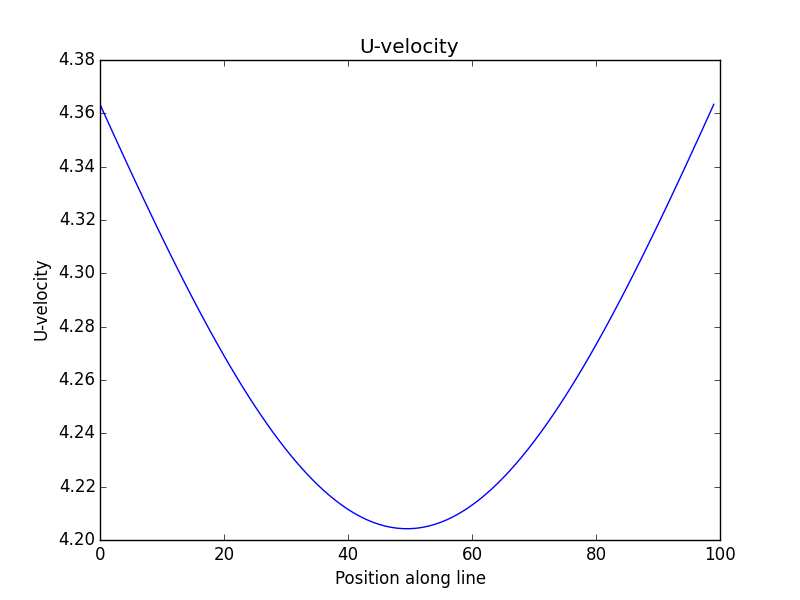
\includegraphics[width=1.0\textwidth]{Figures/U-velocity}
  \caption{x-component of velocity}
\end{subfigure}
\hfill
\begin{subfigure}{0.48\textwidth}
    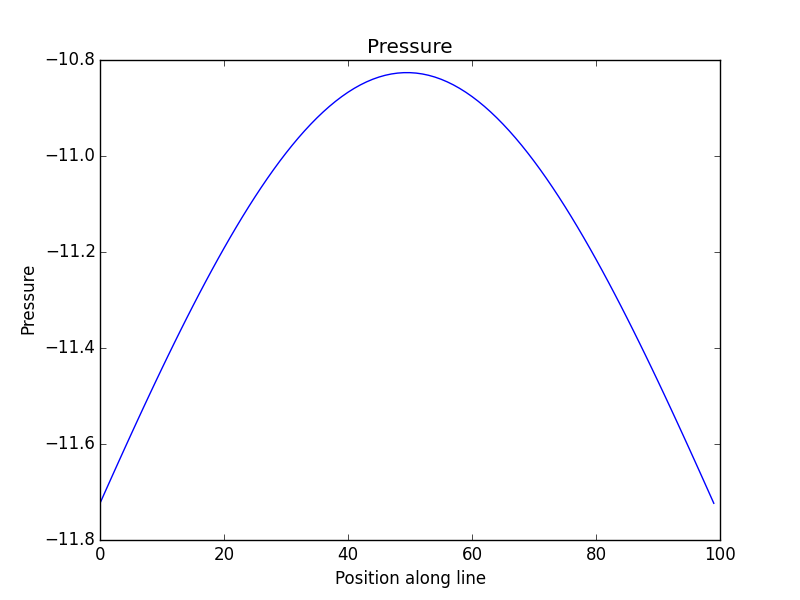
\includegraphics[width=1.0\textwidth]{Figures/P-trace}
  \caption{Pressure}
\end{subfigure}
\caption{Flow properties extracted along straight line between the points (-0.5,-0.5) and (-0.5,0.5).}
\label{F_extract_test}
\end{figure}


The possible options for extracting data are described in section~\ref{S_extract}.


%%%%%%%%%%%%%%%%%%%%%%%%%%%%%%%%%%%%%%%%%%%%%%%%%%%%%%
\subsubsection{Extraction Functions}\label{S_extract}
The following functions extract data from the total flow-field.
They must be executed on the PotentialFlow-filed class (e.g. \verb'T') in the example above.  
In the description below \verb'NAME' is used as a generic placeholder. 
These functions must be executed after \verb'NAME.calc([List])'
\begin{description}
\item[Streamfunction] \verb'Psi = NAME.evalP(x,y)'\\
Returns the total streamfunction magnitude at the point with the coordinates $(x, y)$.

\item[Velocities] \verb' u, v = NAME.eval(x,y)' \\
Returns the $x$ and $y$ component of velocity at the point with the coordinates $(x, y)$.

\item[Pressure] \verb'dP = evalPressure(x,y,rho)'\\
Returns the pressure change relative to ambient conditions (zero velocity)

\item[Line U-Velocity] \verb'UU = LinevalU(x0,y0,x1,y1,n=100,plot_flag=0)' \\
Returns the magnitude of velocity in the x-direction, $u$ at $n$ equally spaced points along the line between the two points $(x0, y0)$ and $(x1,y1)$. 
Setting \verb'plot_flag = 1' will also generate a line graph.

\item[Line V-Velocity] \verb'VV = LinevalV(x0,y0,x1,y1,n=100,plot_flag=0)' \\
Returns the magnitude of velocity in the y-direction, $v$ at $n$ equally spaced points along the line between the two points $(x0, y0)$ and $(x1,y1)$.
Setting \verb'plot_flag = 1' will also generate a line graph.

\item[Line Pressure]  \verb'PP = LinevalPressure(x0,y0,x1,y1,rho,n=100,plot_flag=0)' \\
Returns the pressure change relative to ambient conditions (zero velocity) at $n$ equally spaced points along the line between the two points $(x0, y0)$ and $(x1,y1)$.
Setting \verb'plot_flag = 1' will also generate a line graph.

\end{description}


The following functions extract the flow-field contribution of a single building block. 
They must be executed on the building block class (e.g. \verb'A1') in the example above. 
In the description below \verb'NAME' is used as a generic placeholder.   
\begin{description}
\item[Velocities] \verb' u, v = NAME.eval(x,y)' \\
This returns the $x$ and $y$ component of velocity at the point with the coordinates $(x, y)$.
\end{description}


%%%%%%%%%%%%%%%%%%%%%%%%%%%%%%%%%%%%%%%%%%%%%%%%%%%%%%
%%%%%%%%%%%%%%%%%%%%%%%%%%%%%%%%%%%%%%%%%%%%%%%%%%%%%%
\clearpage
\section{Example - Vortex near wall}
This example shows how \verb'Potential_Flow.py' can be used to analyse the flow field generated by a uniform flow parallel to and a vortex position a distance of \num{0.5} from the wall. 
The problem is illustrated in Fig.~\ref{F_vortex_near_wall_a}.

\begin{figure}[h]
\begin{subfigure}{0.48\textwidth}
    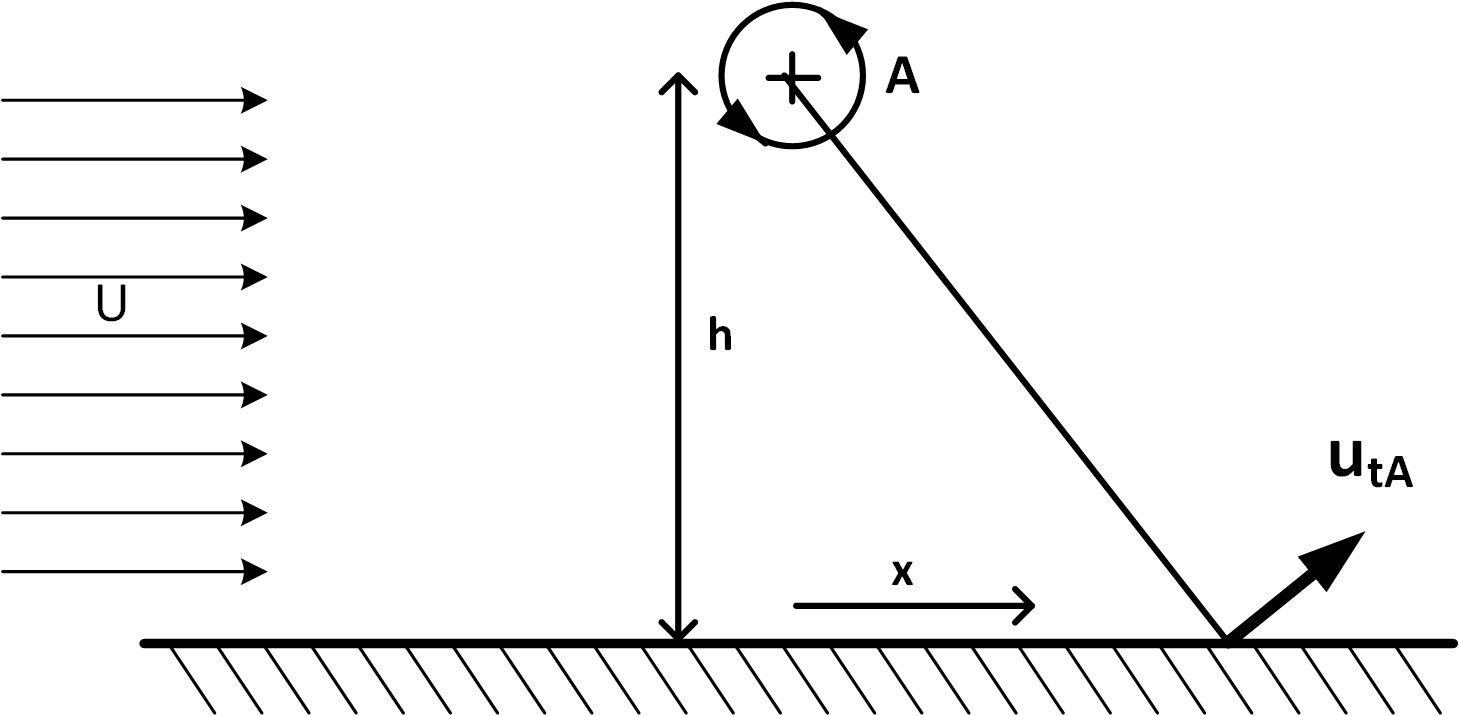
\includegraphics[width=1.0\textwidth]{Figures/Vortex_wall_1}
  \caption{Flow problem}\label{F_vortex_near_wall_a}
\end{subfigure}
\hfill
\begin{subfigure}{0.48\textwidth}
    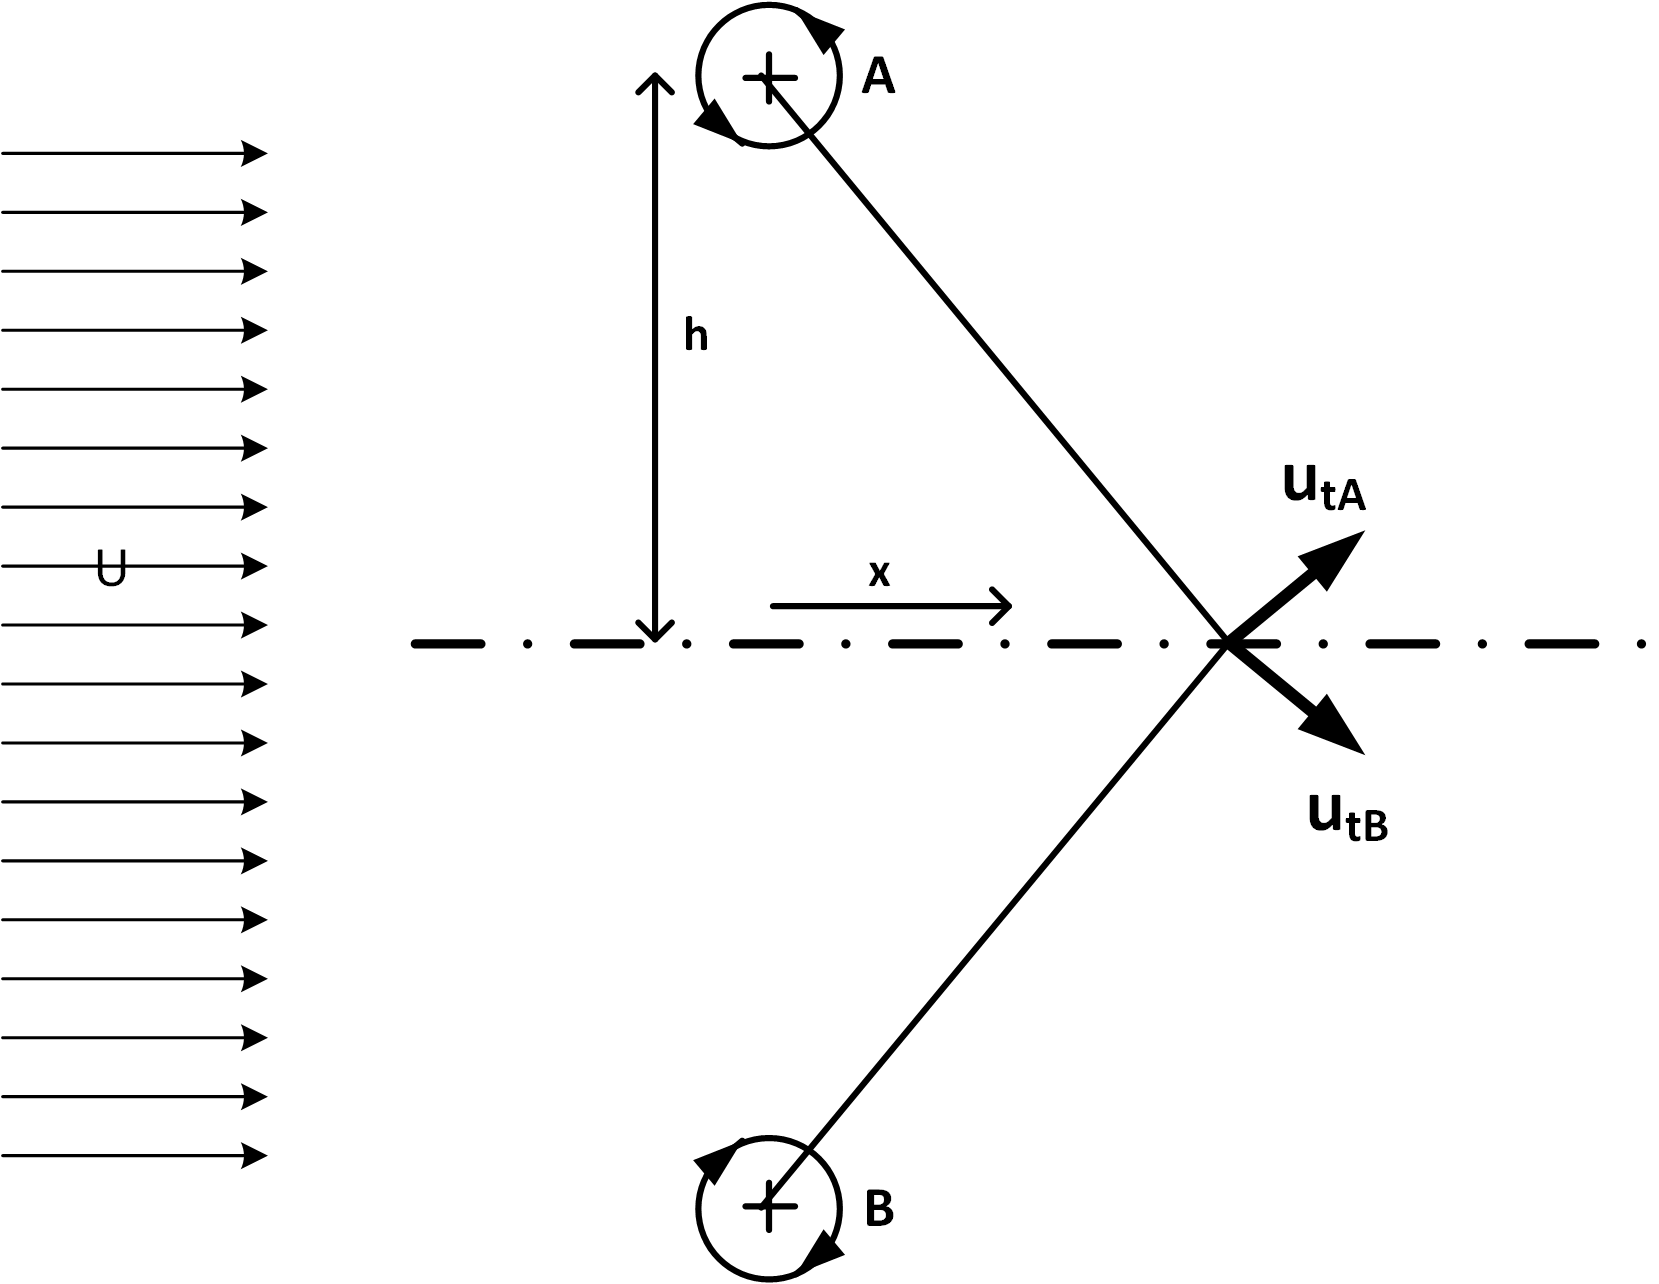
\includegraphics[width=1.0\textwidth]{Figures/Vortex_wall_2}
  \caption{Use aadition of 2nd vortex and use of symetry to create wall}\label{F_vortex_near_wall_b}
\end{subfigure}
\caption{Example case, consisting of uniform flow and a vortex positioned near a wall.}
\label{F_vortex_near_wall}
\end{figure}


In order to generate the effect of a wall (straight streamline) on can use the principle of symmetry.
Thus the problem we will actually solve using Potential Flow theory is the one shown in Fig.~\ref{F_vortex_near_wall_b}, which consists of three building blocks.
The Uniform Flow, the Vortex at $(0.0, 0.5)$ and a mirror image (about the x-axis) of the Vortex, located at $(0.0,-0.5)$, which by symmetry generates a straight streamline along the x-axis. 

The appropriate code, defining the Uniform Flow, with a strength of \num{5.0} and vortices with a strength of $\pm \num{5.0}$ is given below. 
First the building blocks are generated as variables \verb'A1', \verb'C1', and \verb'C2'. 
Then after setting up the flow-field, the list of building blocks \verb'[A1,C1,C2]' is passed to the flow-field solver and evaluated over a $100 \times 100$ grid. 

The results from the plotting functions, showing field data and data along the wall, extracted using the \verb'T.LinevalU', \verb'T.LinevalV' and \verb'T.LinevalPressure ' functions are shown in Fig.~\ref{F_vortex_wall_results}.   
The obtained velocity in the wall parallel direction equals the analytical solution to the problem, given by
\begin{eqnarray}
U_T(x) &=& U_{\infty} +  \frac{ \Gamma \, h}{\pi \left( x^2 + h^2\right) }  \\
\nonumber	& =& \num{5.0}  +  \frac{ \num{5.0} \times \num{0.5} }{\pi \left( x^2 + \num{0.5}^2\right) } \\
\nonumber U_T(0) &=&  \num{5.0} + \num{3.18} = \num{8.18}
\end{eqnarray}


\noindent
\topbar
\begin{lstlisting}
if __name__ == "__main__":

    # List of Building Blocks 
    # Uniform Flows  
    A1 = UniformFlow(5.,0.)
    # Vortices
    C1 = Vortex(0.0,0.5,-5.)
    C2 = Vortex(0.0,-0.5,5.)

    # Initialise instance of Plotting Function
    T = PlotPotentialFlow()   	# create instance of the PotentialFlow-field class
    # Set dimensions of Plotting area
    T.size(-2.0, 2.0, -1.0 ,1.0)   #(x_min, x_max, y_min, y_max)

    # Evaluate PotentialFlow-field over a grid
    T.calc([A1,C1,C2],n=100)   # ([List of elements], level of discretisation)

    # plot Data over flow-field area
    T.plot_Streamlines()    # create Streamline plot.
    T.plot_P(P_inf = 0., rho=1.225, P_min=-100., P_max=200.)   # create plot of Pressure contours

    # extract data at points
    # print 'Psi = ', T.evalP(0.,0.)
    print '(u, v) = ', T.eval(0.,0.)
    print 'dP = ', T.evalPressure(0.,0.,rho = 1.225)

    # extact data along lines 
    # lines are defined as x0,y0,x1,y1
    T.LinevalU(-2.0,0.0,2.0,0.0,plot_flag=1)
    T.LinevalV(-2.0,0.0,2.0,0.0,plot_flag=1)
    T.LinevalPressure(-2.0,0.0,2.0,0.0,rho = 1.225, plot_flag=1)

    # Make sure plots are displayed on the screen
    plt.show()
\end{lstlisting}
\bottombar

The resulting data is shown in Fig.~\ref{F_vortex_near wall}. 
In addition the following data, corresponding to point extractions is displayed on screen: \\
\verb'(u, v) = (8.1830988, 0.0)' \\
\verb'dP = -41.0149'

These correspond to the $u$ and $v$-velocity components. 
Obviously $v=0$ along the wall and $u=8.18$, which agrees with the analytical solution for this point.  
Similar \verb'dP' gives the pressure reduction, calculate as $\Delta P = - \frac{1}{2} \, \rho \, U^2 = -41.01$. 


\begin{figure}
\centering
\begin{subfigure}{0.48\textwidth}
    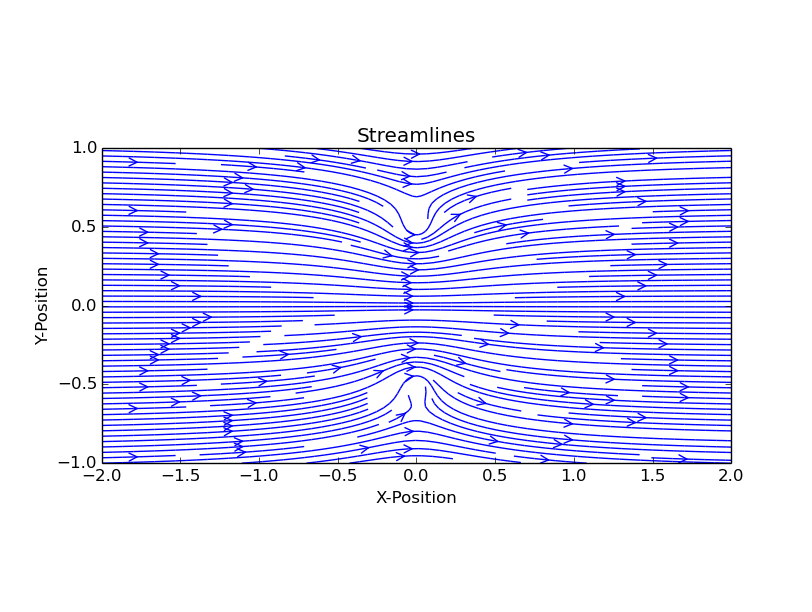
\includegraphics[width=1.0\textwidth]{Figures/Vortex_wall_SL}
  \caption{Streamlines}
\end{subfigure}
\hfill
\begin{subfigure}{0.48\textwidth}
    \includegraphics[width=1.0\textwidth]{Figures/Vortex_wall_pressure}
  \caption{Pressure contours}
\end{subfigure} \\
\centering
\begin{subfigure}{0.48\textwidth}
    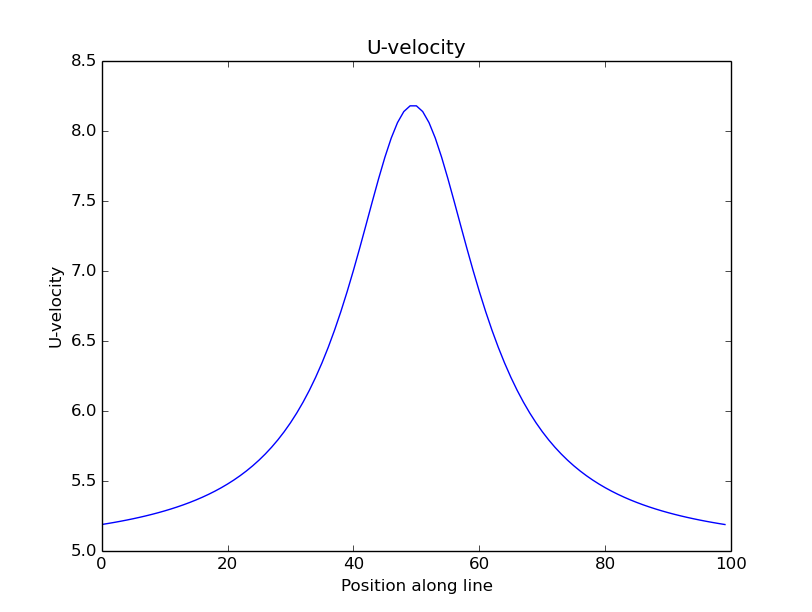
\includegraphics[width=1.0\textwidth]{Figures/Vortex_wall_U}
  \caption{U-Velocity, extracted along the x-axis}
\end{subfigure}
\hfill
\begin{subfigure}{0.48\textwidth}
    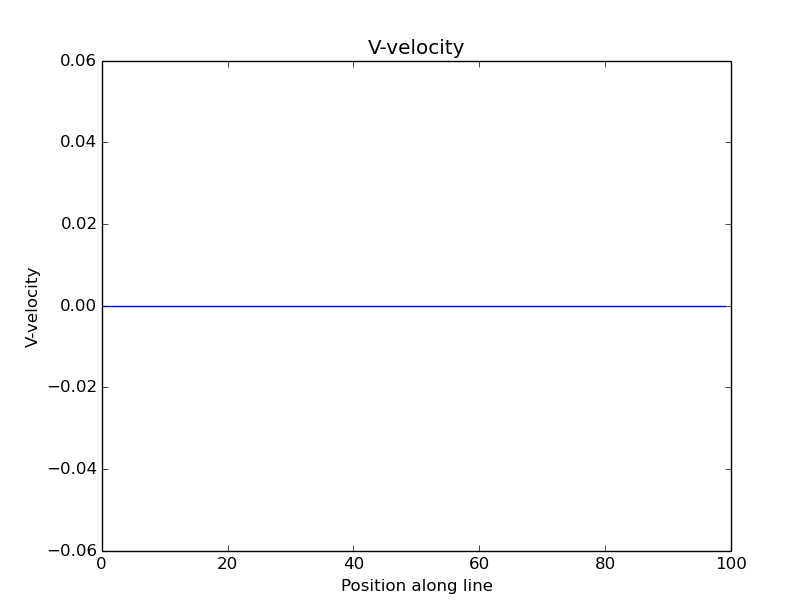
\includegraphics[width=1.0\textwidth]{Figures/Vortex_wall_V}
  \caption{V-velocity, exteacted along the x-axis}
\end{subfigure} \\
\centering
\begin{subfigure}{0.48\textwidth}
    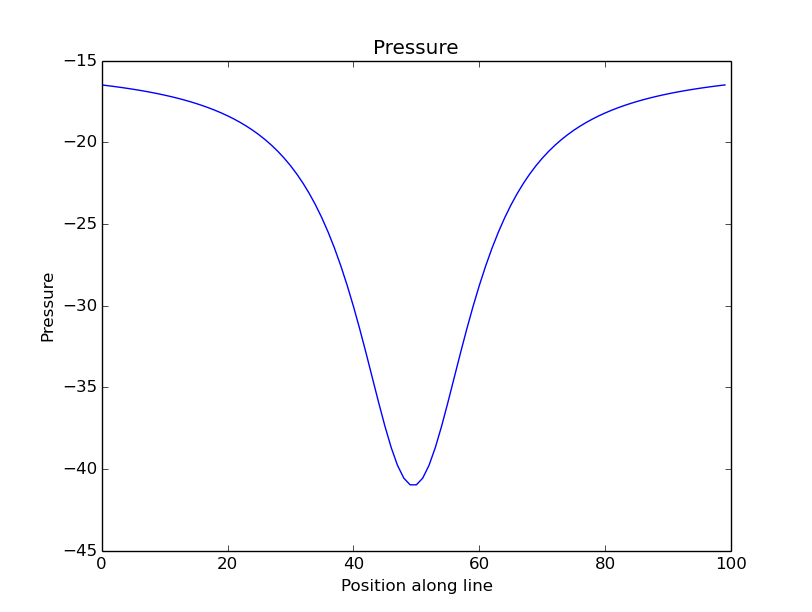
\includegraphics[width=1.0\textwidth]{Figures/Vortex_wall_P_wall}
  \caption{Static Pressure, extracted along the x-axis}
\end{subfigure}
\hfill
\caption{Flow field and flow properties obtained from a uniform flow with $u$-velocity of \num{5.0} and a vortex with a strength of \num{-5.0} positioned $(0.0, 0.5)$ positioned near a wall running along the x-axis as shown.}
\label{F_vortex_wall_results}
\end{figure}




%%%%%%%%%%%%%%%%%%%%%%%%%%%%%%%%%%%%%%%%%%%%%%%%%%%%%%
%%%%%%%%%%%%%%%%%%%%%%%%%%%%%%%%%%%%%%%%%%%%%%%%%%%%%%
\clearpage
\section{References}

\begin{thebibliography}{9}
\bibitem[CFCFD (2015)]{cfcfdpage:2015} 
CFCFD,
\emph{The Compressible Flow Project}
\url{http://cfcfd.mechmining.uq.edu.au}
The University of Queensland

\end{thebibliography}

%%%%%%%%%%%%%%%%%%%%%%%%%%%%%%%%%%%%%%%%%%%%%%%%%%%%%%
%%%%%%%%%%%%%%%%%%%%%%%%%%%%%%%%%%%%%%%%%%%%%%%%%%%%%%
\section{Appendix}


%%%%%%%%%%%%%%%%%%%%%%%%%%%%%%%%%%%%%%%%%%%%%%%%%%%%%%
\subsection{Source Code Potential\textunderscore Flow.py}

\noindent

\lstset{language=python,
%    basicstyle = \small,
    basicstyle = \footnotesize,
%    keywordstyle=\color{brown},
%    stringstyle=\color{pink},
%    commentstyle=\color{blue},
%    morecomment=[l]{#},
%    morecomment=[n]{'''}{'''},
    showstringspaces=false,
    numbers=left,
    numberstyle=\tiny,
    numbersep=2pt,
    breaklines=true
}

\noindent
\topbar
\lstinputlisting{Code/Potential_Flow.py}
\bottombar



\end{document}
